%%%%%%%%%%%%%%%%%%%%%%%%%%%%%%%%%%%%%%%%%%%%%%%%%%%%%%%%%%%%%%%%%%%%%%%%%%%%%%%%%%
\begin{frame}[fragile]\frametitle{}
\begin{center}
{\Large Random Variables}
\end{center}
\end{frame}

%%%%%%%%%%%%%%%%%%%%%%%%%%%%%%%%%%%%%%%%%%%%%%%%%%%%%%%%%%
\begin{frame}\frametitle{Random Variables}
\begin{itemize}
\item Random Variables, is actually a misnomer. They are not variables in the programming sense. They are Functions mapping outcomes of Random Processes to real numbers.
\item Example:
\begin{itemize}
\item Random Process: Coin flipping
\item Outcomes: HEAD or TAIL
\item Real numbers: 1 for HEAD and 0 for TAIL
\end{itemize}

\item Another Example:
\begin{itemize}
\item Random Process: rolling of 7 dice
\item Outcomes: take top numbers of each
\item Real numbers: Sum of the top numbers
\end{itemize}
\item Whats the use of doing this?
\item Gives easy way to express the random processes, in an equation.
\end{itemize}
\end{frame}

%%%%%%%%%%%%%%%%%%%%%%%%%%%%%%%%%%%%%%%%%%%%%%%%%%%%%%%%%%
\begin{frame}\frametitle{Random Variables}
\begin{itemize}
\item Example: Find probability of sum of top of 7 dice being less than 30.
If $Y$ is said to represent ``sum of top of 7 dice'' then it can be expressed as $P(Y \leq 30)$.
\item Similarly, Random variables allows us to ask questions in mathematical way.
If we flip 5 coins and want to answers questions like:
\begin{itemize}
\item What is the probability of getting exactly 3 heads?
\item What is the probability of getting less than 4 heads?
\item What is the probability of getting more than 1 head?
\end{itemize}
\item Then our general way of writing would be:
\begin{itemize}
\item P(Probability of getting exactly 3 heads when we flip a coin 5 times)
\item P(Probability of getting less than 4 heads when we flip a coin 5 times)
\item P(Probability of getting more than 1 head when we flip a coin 5 times)
\end{itemize}
\item But if we use random variables to represent above questions then we would write:
\begin{itemize}
\item $P(X=3)$
\item $P(X<4)$
\item $P(X>1)$
\end{itemize}
\item As we can see above random variables makes our task much easier to quantify results of any random process and apply math and perform further computation.
\end{itemize}
\end{frame}

%%%%%%%%%%%%%%%%%%%%%%%%%%%%%%%%%%%%%%%%%%%%%%%%%%%%%%%%%%
\begin{frame}\frametitle{Random Variables}
\begin{itemize}

\item Intuitively, those variables which can take different, unpredictable values are called
random variables.
\item A Random Variable is different from the variable in algebra as it has whole set of values and it can take any of those randomly. Variable used in algebra cannot have more than a single value at a time.
\item If random variable $X={0,1,2,3}$. Then $X$ could be 0, 1, 2 or 3 randomly where each of them might have a different probability.
\item We use capital letter for random variables to avoid confusion with traditional variables.
\item If the variables are discrete in nature, they are called discrete random
variables. Example: In an experiment of tossing 2 coins, we need to find out the possible number of heads. Therefore $X= {0, 1, 2}$
\item Similarly, if the variables are continuous in nature, then it is called
continuous random variable. Example: temperature in a city lies between 30C and 45C centigrade. The temperature can take any value in the interval 30C to 45C.
\end{itemize}
\end{frame}

%%%%%%%%%%%%%%%%%%%%%%%%%%%%%%%%%%%%%%%%%%%%%%%%%%%%%%%%%%
\begin{frame}\frametitle{Mathematically, Random Variable}
\begin{itemize}

\item A (real-valued) random variable, often denoted by $X$ (or some other capital letter), is a function mapping a probability space $(S, P)$ into the real line ${\mathbb R}$
\item Associated with each point $s$ in the domain $S$ the function $X$ assigns one and only one value $X(s)$ in the range ${\mathbb R}$

\begin{center}
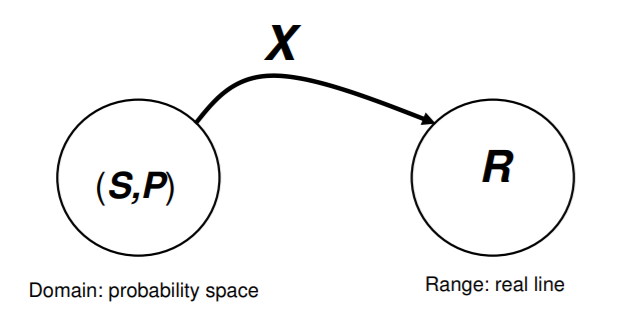
\includegraphics[width=0.6\linewidth,keepaspectratio]{random1}
\end{center}

\item As such, a random variable has a probability distribution. $P$ is the probability measure on the underlying sample space $S$
\end{itemize}

\tiny{(Ref: IEOR 4106: Introduction to Operations Research: Stochastic Models)}

\end{frame}

%%%%%%%%%%%%%%%%%%%%%%%%%%%%%%%%%%%%%%%%%%%%%%%%%%%%%%%%%%
\begin{frame}\frametitle{Function of a Random Variable}
\begin{itemize}

\item Suppose that we are given a random variable $X$ mapping
the probability space $(S, P)$ into the real line ${\mathbb R}$ and we are given a function $h$ mapping ${\mathbb R}$ into ${\mathbb R}$. 
\item Then $h(X)$ is a function mapping the probability space $(S, P)$ into ${\mathbb R}$. 
\item As a consequence, $h(X)$ is itself a new random variable, i.e., a new function mapping $(S, P)$ into ${\mathbb R}$

\begin{center}
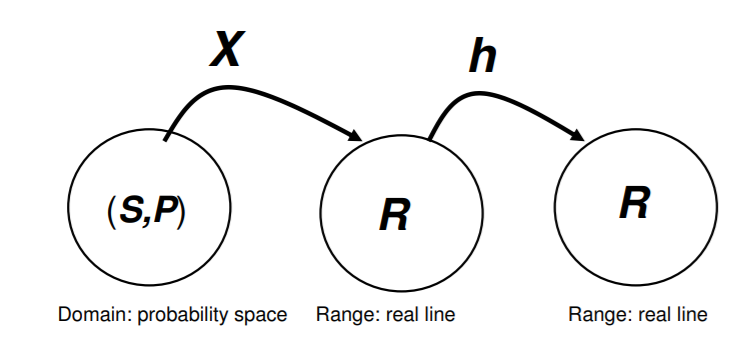
\includegraphics[width=0.6\linewidth,keepaspectratio]{random2}
\end{center}


\end{itemize}

\tiny{(Ref: IEOR 4106: Introduction to Operations Research: Stochastic Models)}

\end{frame}



%%%%%%%%%%%%%%%%%%%%%%%%%%%%%%%%%%%%%%%%%%%%%%%%%%%%%%%%%%
\begin{frame} \frametitle{Random variables}
A {\bf random variable} is generated by a ``random'' function. 

Types:
\begin{itemize}
\item Nominal
\item Ordinal
\item Quantitative
\end{itemize}
\end{frame}


%%%%%%%%%%%%%%%%%%%%%%%%%%%%%%%%%%%%%%%%%%%%%%%%%%%%%%%%%%
\begin{frame}\frametitle{Nominal Random Variable}
\begin{itemize}
\item A {\bf nominal} random variable, also called {\bf qualitative} or {\bf  categorical}, takes on values in a set of names or labels.
\item Examples of nominal sample spaces include geographical locations, biological species, and ethnic categories.
\item Data from a nominal random variable cannot be {\bf strictly ordered}.
\end{itemize}
\end{frame}

%%%%%%%%%%%%%%%%%%%%%%%%%%%%%%%%%%%%%%%%%%%%%%%%%%%%%%%%%%
\begin{frame}\frametitle{Ordinal Random Variable}

\begin{itemize}
\item An {\bf ordinal} measurement is usually either a {\bf ranking}
($1^{\rm st}$, $2^{\rm nd}$, etc.) or a {\bf rating} (good, bad,
favorable, strongly agree, etc.).  

\item Ordinal values can be ordered, but do not have {\bf measurement units}
\item It doesn't always make sense to subtract or divide their numerical
values.
\end{itemize}
\end{frame}

%%%%%%%%%%%%%%%%%%%%%%%%%%%%%%%%%%%%%%%%%%%%%%%%%%%%%%%%%%
\begin{frame}\frametitle{Quantitative Random Variable}

\begin{itemize}
\item A {\bf quantitative} random variable represents a magnitude, for
example the result of counting something, or the result of measuring a
physical quantity such as length, width, or volume.

\item Quantitative measurements can always be ordered.
\end{itemize}
\end{frame}

%%%%%%%%%%%%%%%%%%%%%%%%%%%%%%%%%%%%%%%%%%%%%%%%%%%%%%%%%%%
%\begin{frame}
%\frametitle{Measurement scales}
%
%\begin{itemize}
%\item Celsius temperature is an interval scale -- it makes
%perfect sense to compare two temperatures by subtracting them.
%\item Is Celsius temperature a ratio scale?  Is the coffee twice as hot as
%the tea?
%\item 
%The answer is no.  The freezing point of water defines the origin of
%the Celsius scale.  This is arbitrary.  Pure ethanol freezes at
%$-114^\circ$C, so if we used the freezing point of ethanol as the zero
%point of the scale, the ratio between the two objects' temperatures
%would be only $(50+114)/(25+114)=1.2$.
%
%\textcolor{blue}{Note:} There is some ambiguity and controversy about
%these designations.
%
%\end{frame}

%%%%%%%%%%%%%%%%%%%%%%%%%%%%%%%%%%%%%%%%%%%%%%%%%%%%%%%%%%%
\begin{frame}
\frametitle{ Quantitative Random Variable }
Types:
\begin{itemize}
\item Discrete: Number of days that it rains yearly 
\item Continuous:  Amount of rain on a given day 
\end{itemize}
Note that these designations aren't used in the case of nominal or
ordinal random variables.
\end{frame}

%%%%%%%%%%%%%%%%%%%%%%%%%%%%%%%%%%%%%%%%%%%%%%%%%%%%%%%%%%%
\begin{frame}
\frametitle{ Quantitative Random Variable }

\begin{itemize}
\item A {\bf discrete} random variable takes on finitely many values, or
infinitely many separated values (e.g.\ $0,1,2,\ldots$).

\item A {\bf continuous} random variable can take on any real number in some
interval (e.g.\ $[0,1]$ or $[0,\infty)$).  

\item Gray area between discrete and continuous random variables:
e.g.\ monetary values recorded in dollars or dollars and cents
\end{itemize}
\end{frame}

%%%%%%%%%%%%%%%%%%%%%%%%%%%%%%%%%%%%%%%%%%%%%%%%%%%%%%%%%%%
\begin{frame}
\frametitle{Units, populations and samples}

\begin{itemize}
\item A {\bf unit} (more specifically {\bf ``sampling unit''}) is one member
of the collection.
\item A {\bf population} is the set of all units of interest. 
\item In practice, we cannot observe the whole population, so we usually
work with a {\bf sample} of units
\end{itemize}
\end{frame}

%%%%%%%%%%%%%%%%%%%%%%%%%%%%%%%%%%%%%%%%%%%%%%%%%%%%%%%%%%%
\begin{frame}
\frametitle{Units, populations and samples}

%\textcolor{blue}{\bf Example:} Suppose we are interested in childrens'
%diets, and we sample 100 seven year old
%girls in the US and record their food intake for one day.

\begin{itemize}
\item Properties of a sample will generally differ from properties of the
population.  
\item For example, the 100 children in our sample may have
somewhat higher or somewhat lower average calorie intake than the
population at large. 
\item 
Statistics: how samples relate to
populations, and what we can confidently state about a population
given the limited information in a sample.

\end{itemize}

\end{frame}

%%%%%%%%%%%%%%%%%%%%%%%%%%%%%%%%%%%%%%%%%%%%%%%%%%%%%%%%%%
\begin{frame}\frametitle{Random Variables}
\begin{itemize}
\item  Random variable can take on randomly different
value. 
\item But are all the values that it takes can be equal or likely be equal
too, or is it more likely that the random variable take a particular value
more often than other?
\item Depends on the way (function) using which random numbers are generated.
\end{itemize}
\end{frame}

%%%%%%%%%%%%%%%%%%%%%%%%%%%%%%%%%%%%%%%%%%%%%%%%%%%%%%%%%%
\begin{frame}\frametitle{Random Variable Generation}
\begin{itemize}
\item  Experiment: records numbers from a SINGLE six face die.
\item X axis shows 6 possible outcomes.
\item Y axis shows their probabilities.
\item For each of the 6 possible values on X axis, the Y value is same ie 1/6
\item Uniform distribution
\end{itemize}
\end{frame}

%%%%%%%%%%%%%%%%%%%%%%%%%%%%%%%%%%%%%%%%%%%%%%%%%%%%%%%%%%
\begin{frame}\frametitle{Random Variable Generation}
\begin{itemize}
\item  Experiment: records sum of numbers from TWO six face dies.
\item X axis shows 12 possible outcomes.
\item Y axis shows their probabilities.
\item For each of the 12 possible values on X axis, the Y value is NOT SAME.
\end{itemize}

\begin{center}
\includegraphics[width=0.5\linewidth,keepaspectratio]{pmf}
\end{center}
\end{frame}

%%%%%%%%%%%%%%%%%%%%%%%%%%%%%%%%%%%%%%%%%%%%%%%%%%%%%%%%%%
\begin{frame}\frametitle{Random Variable Generation}
\begin{itemize}
\item  If the random variable is discrete in nature, we use Probability Mass
Function to describe its probability distribution
\item If the random variable is continuous in nature, we use Probability
Density Function to describe its probability distribution.
\end{itemize}
\end{frame}
